\section{Tectonic seismic regions and seismicity parameters}
\noindent
The Iranian plateau is located on the Himalayan-Alpine seismic belt. It has a long history of large magnitude ($M>7$) earthquakes that are well documented dating back to the eighth century. Based on seismicity parameters and the geologic provinces of the plateau, Iranian earthquakes have been categorized into various seismic zones, ranging from the definition of four to nine major seismic zones in the more traditional studies \citep[e.g.,][]{Stocklin1968,Takin1972,Berberian1976}, and up to twenty to twenty-three tectonic seismic regions in the most elaborate ones \citep[e.g.,][]{Nowroozi1976,Tavakoli1999}. \citet{Mirzaei1998},  dividing Iran into five tectonic regions, called Azerbaijan-Alborz, Kopeh-Dagh, Zagros, Central-East Iran, and Makran. Considering the division of  \citet{Mirzaei1998} as a reference,  \citet{Karimiparidari2013}  divided the Azerbaijan-Alborz tectonic seismic region into two regions, which are Azerbaijan and the Alborz Mountain Range (hereinafter, Alborz). Azerbaijan, Alborz, and Kopeh-Dagh tectonic seismic regions encompass most of northern Iran.  Fig.~\ref{fig:study_region} shows the study area and tectonic seismic regions. \\
 
\begin{figure} [ht]
\centering
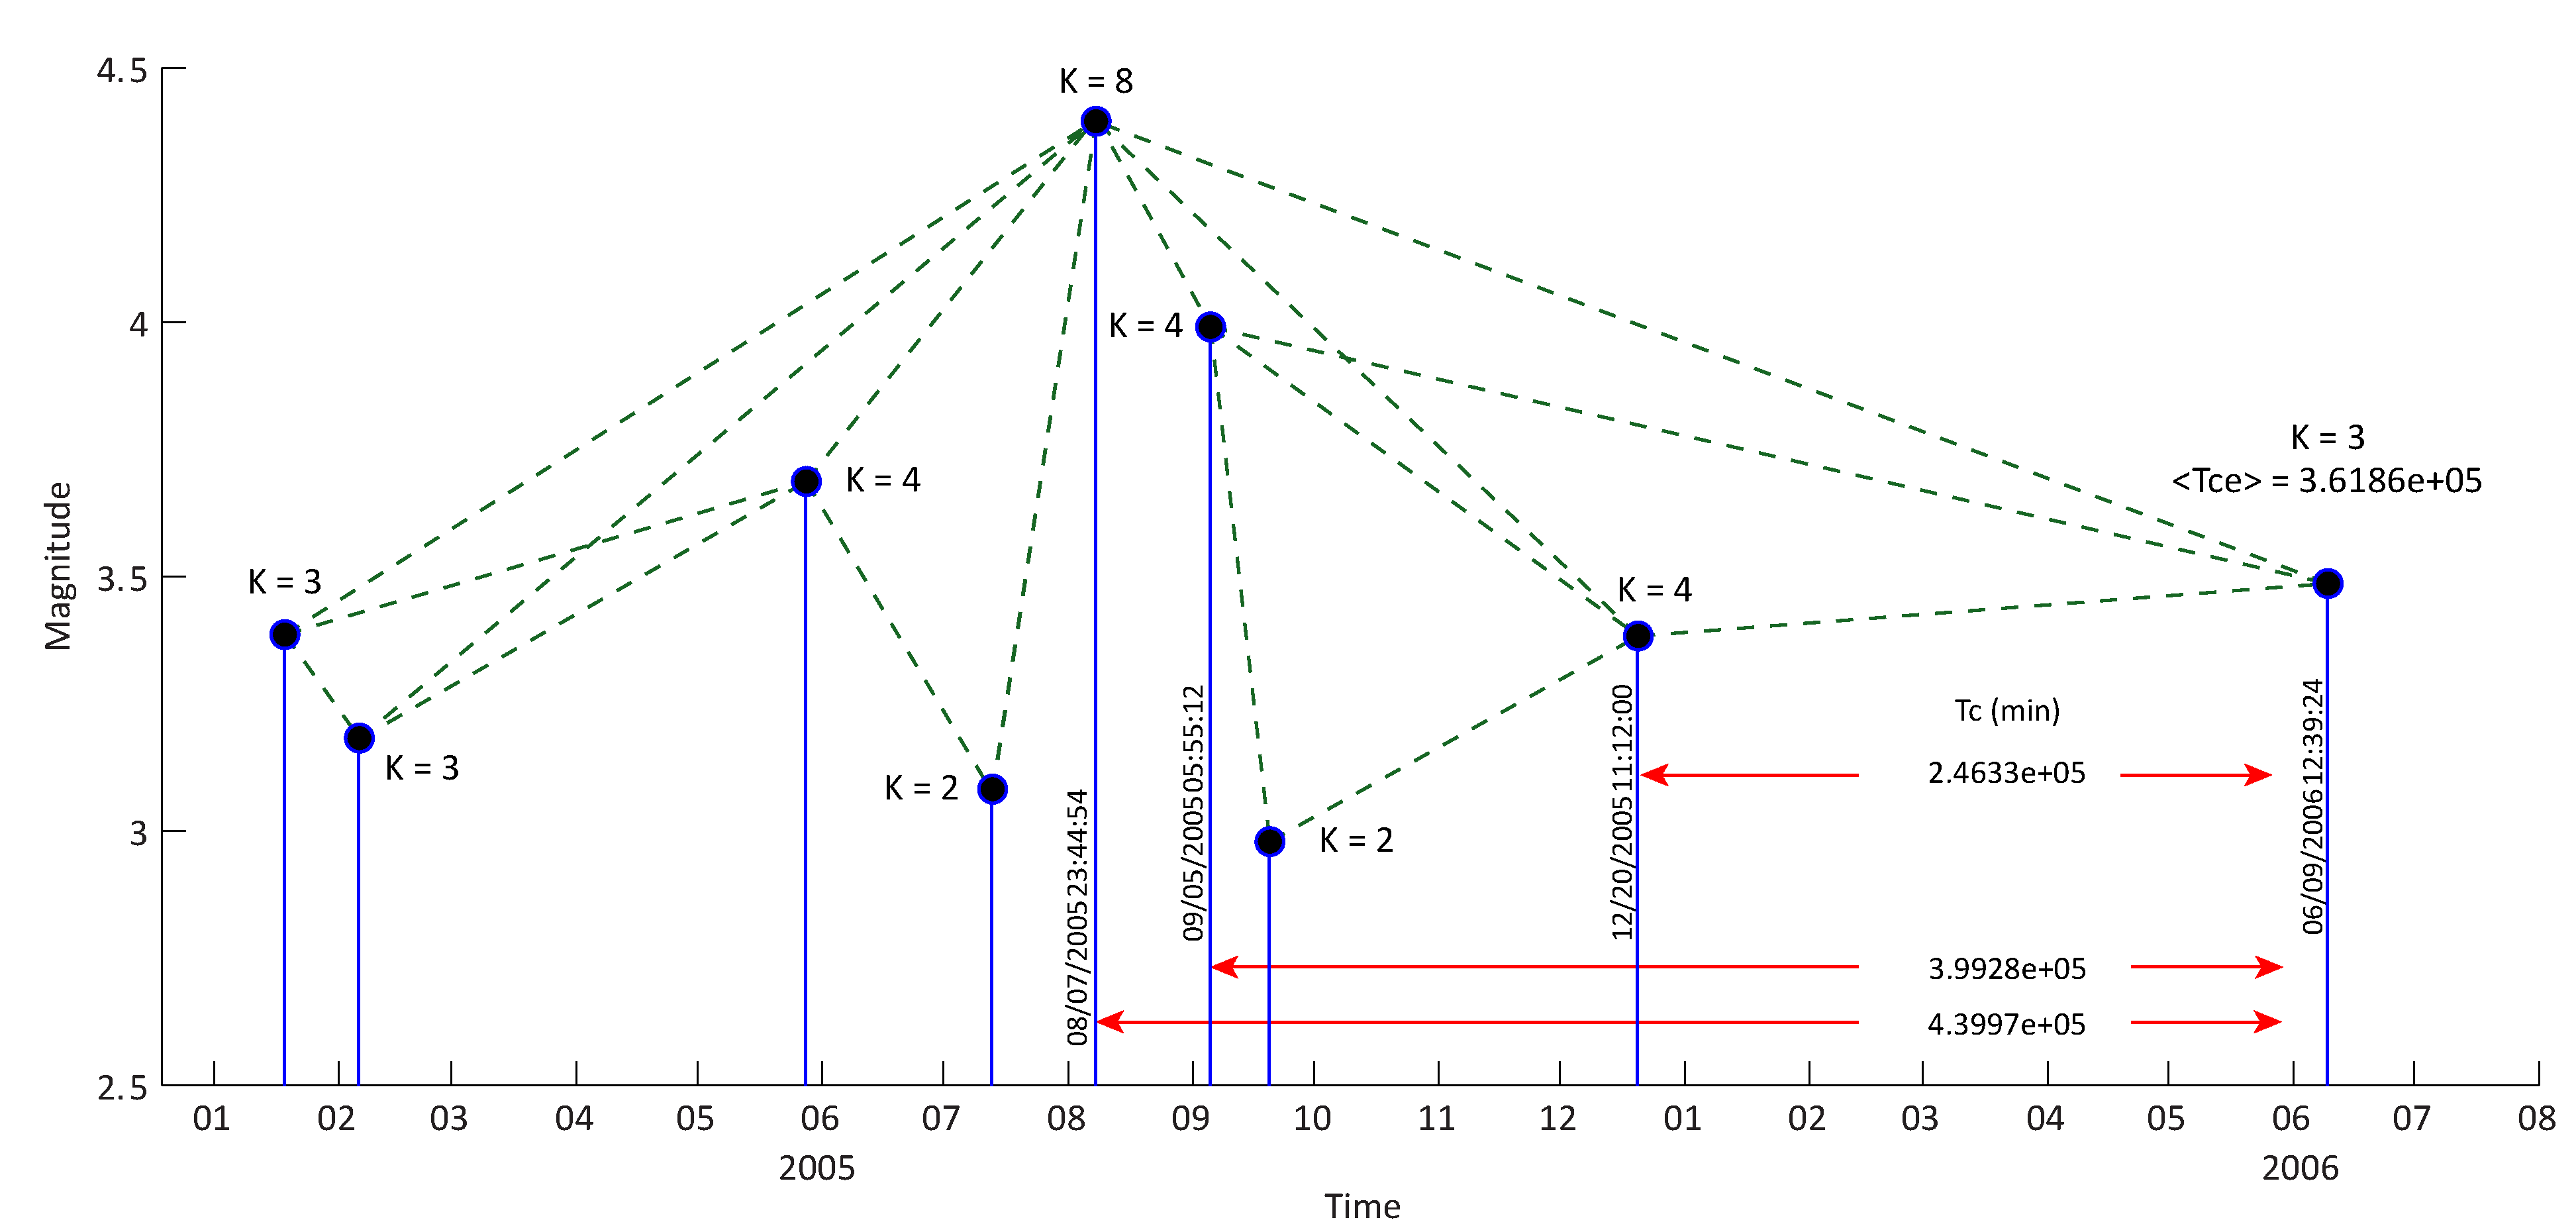
\includegraphics[scale=1]{figures/pdf/Figure01.pdf} 
\caption{Region of interest and tectonic seismic regions. At the top, the map of Iran and surrounding countries is presented. The study area is located in the gray box. At the bottom, the study area containing seismotectonic provinces after \citet{Mirzaei1998} is presented. Dashed line is the subdivision that is proposed by \citet{Karimiparidari2013}}
\label{fig:study_region}
\end{figure}
  
\noindent
The Alborz tectonic seismic region has active reverse faults, which are parallel to the northwest-trending structural gain of the Alborz Mountains belt. The North Tehran Thrust adds more complexity due to the presence of south-dipping reverse faults, which are in part blind, such as the Davudieh, Shian, and Bagh-E Feyz. The northwest continuation of the Alborz Mountains, known as the Rocks of the Talesh Mountains, have been thrust northeastward and eastward over rocks of the south Caspian depression  \citep{Berberian1999}.\\ 
\noindent
The Tabriz region (located in the Azerbaijan tectonic seismic region) is in the Araxes structural block of northwestern Iran, southwest of the continuation of the western Alborz Mountains toward the Caucasus. The North Tabriz Fault (NTF) is a complex northwest-trending structure, which contains evidence observed on aerial photographs, and vertical displacement with the north side up, of right-lateral strike-slip displacement  \citep{Berberian1999}.
\noindent
The main Kopeh-Dagh fault consists of several partly overlapping segments parallel to the overall  NW - SE  structure with step-overs. The regions of overlap are characterized by shorter south-dipping thrust faults, striking roughly E - W  \citep{Berberian2001}.  \citet{Trifonov1978}  reported active displacement along the main Kopeh-Dagh fault for more than 500 km. Main fault lines and fault systems in the interest region is represented in Fig.~\ref{fig:faults}.


\begin{figure} [ht]
\centering
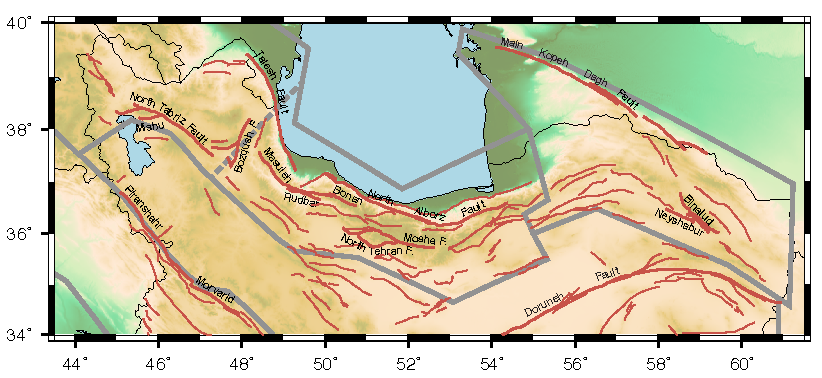
\includegraphics[scale=1]{figures/pdf/Figure02.pdf} 
\caption{Main fault line and fault system in the region of interest. The borderlines of the seismic zones shown in Fig.~\ref{fig:study_region} are shown in background in gray.}
\label{fig:faults}
\end{figure}


\subsection{Magnitude Conversion}
\noindent
The catalog of recorded earthquakes from 2005-15, downloaded from IIEES, reported earthquakes based on different magnitude scales \citep{IIEES}. The  $M_L$,  $M_S$, and  $mb$  magnitudes were converted through conversion relationships, as defined in  \citet{Zare2014}. Some data were also recorded in  $M_D$  (duration magnitude). These data are reported by the International Seismological Centre (ISC).   \citet{Deniz2010}  developed a set of empirical equations to convert earthquake magnitudes from  $mb$,  $M_D$,  $M_L$, and  $M_S$  scales to  $M_W$  scale using the orthogonal regression procedure. They used data from different data centers, including the ISC, of earthquakes that occurred in Turkey. In this study, we use the conversion equation of  \citet{Deniz2010}  to convert  $M_D$  to  $M_W$. 

\subsection{Declustering} 
\noindent
It is generally assumed that the seismicity of each tectonic seismic source follows a Poissonian occurrence process. Therefore, in order to accomplish this, we decluster the earthquake catalog. In compiling the catalog of events, foreshocks and aftershocks are removed using a declustering methodology  presented by \citet{Gardner1974}. Fig.~\ref{fig:seismicity}  shows the epicenter of declustered instrumental  earthquakes.

\begin{figure} [ht]
\centering
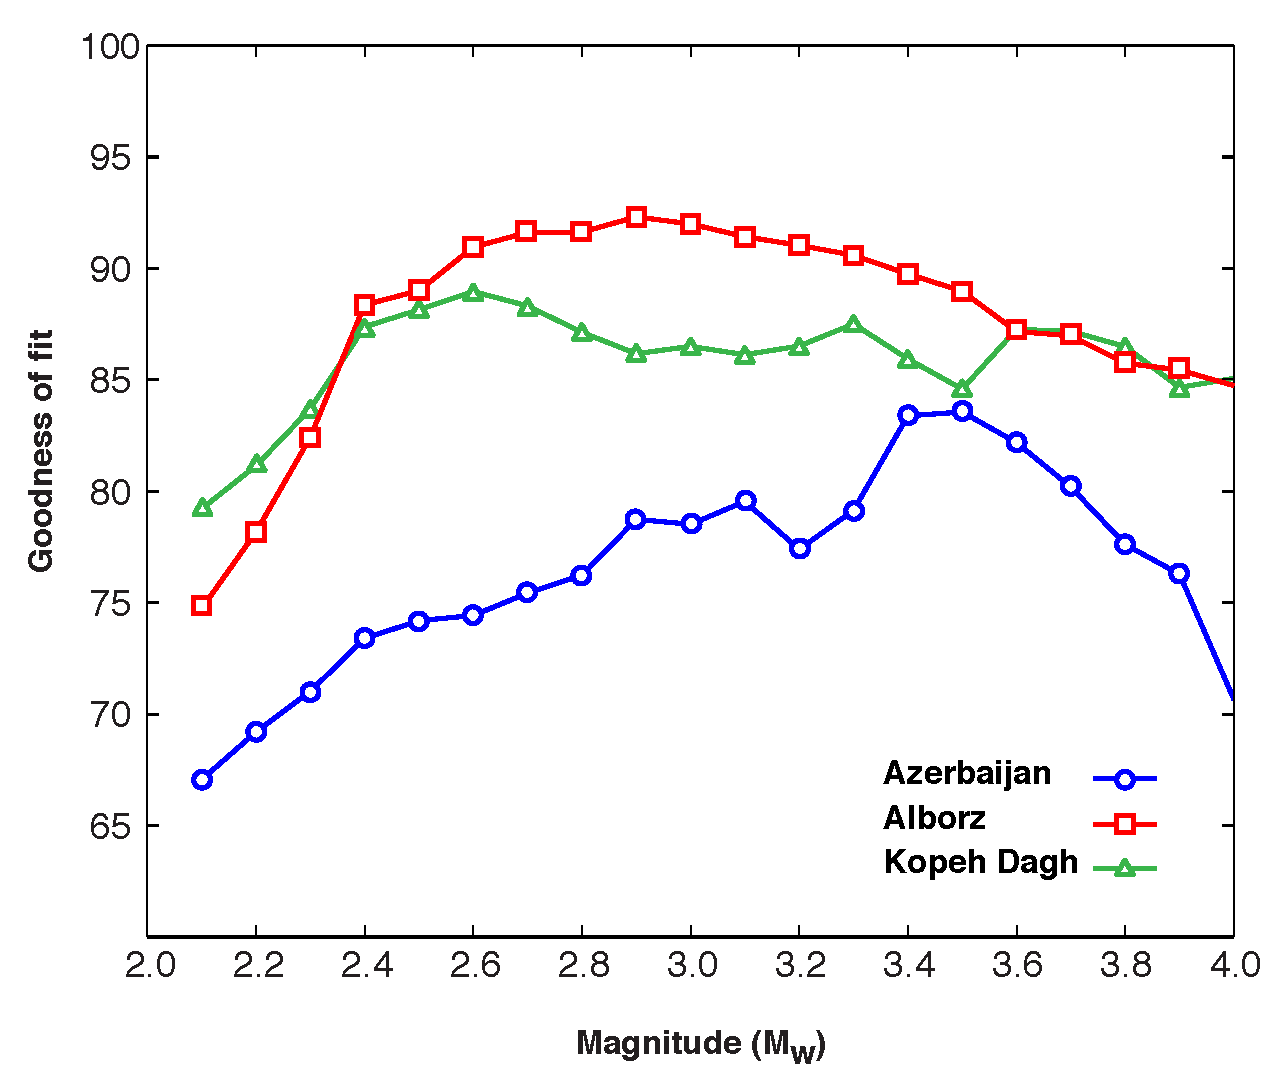
\includegraphics[scale=1]{figures/pdf/Figure03.pdf} 
\caption{Declustered instrumental seismicity map (2005 - 2015) of northern Iran. Different colors indicate the seismicity of different regions. Size of symbols are proportional to the magnitude of the events.}
\label{fig:seismicity}
\end{figure}


 
\subsection{Catalog Completeness}
\noindent
Catalog completeness is an important factor in studying an earthquake sequence. This characteristic measured as the minimum magnitude of complete recording for earthquake catalog. The completeness magnitude $(M_c)$ is often determined using simple numerical analysis. Two common approaches are maximum curvature method and (MAXC) and goodness-of-fit test (GFT)(see \citet{Wiemer2000}). We use the Goodness-of-fit test and compute $M_c$ for each region's catalog. According to the GFT method, a complete catalog should follow the Gutenberg-Richter power law distribution of magnitude. The steps for selecting the completeness magnitude for each catalog include: 1) calculating the a-  and  b-  value based on minimum magnitude; 2) generating  synthetic events based on the achieved value when the cumulative number of events obey the power law distribution; and 3) calculating goodness of fit for predicted and observed cumulative numbers for each magnitude bin  \citep{Wiemer2000}. We increase the minimum magnitude and repeat the process in order to calculate the goodness of fit for each magnitude.  \citet{Wiemer2000} assumed a goodness of fit of 90\% as a threshold to select the completeness of the catalog. However,  not all frequency-magnitude distributions reach the 90\% mark. Fig.~\ref{fig:completeness} shows the goodness-of-fit values for three tectonic seismic regions. For each tectonic seismic region, we select the magnitude corresponding to the highest goodness of fit or the first magnitude with the goodness of fit greater than 90\%.

\begin{figure} [ht]
\centering
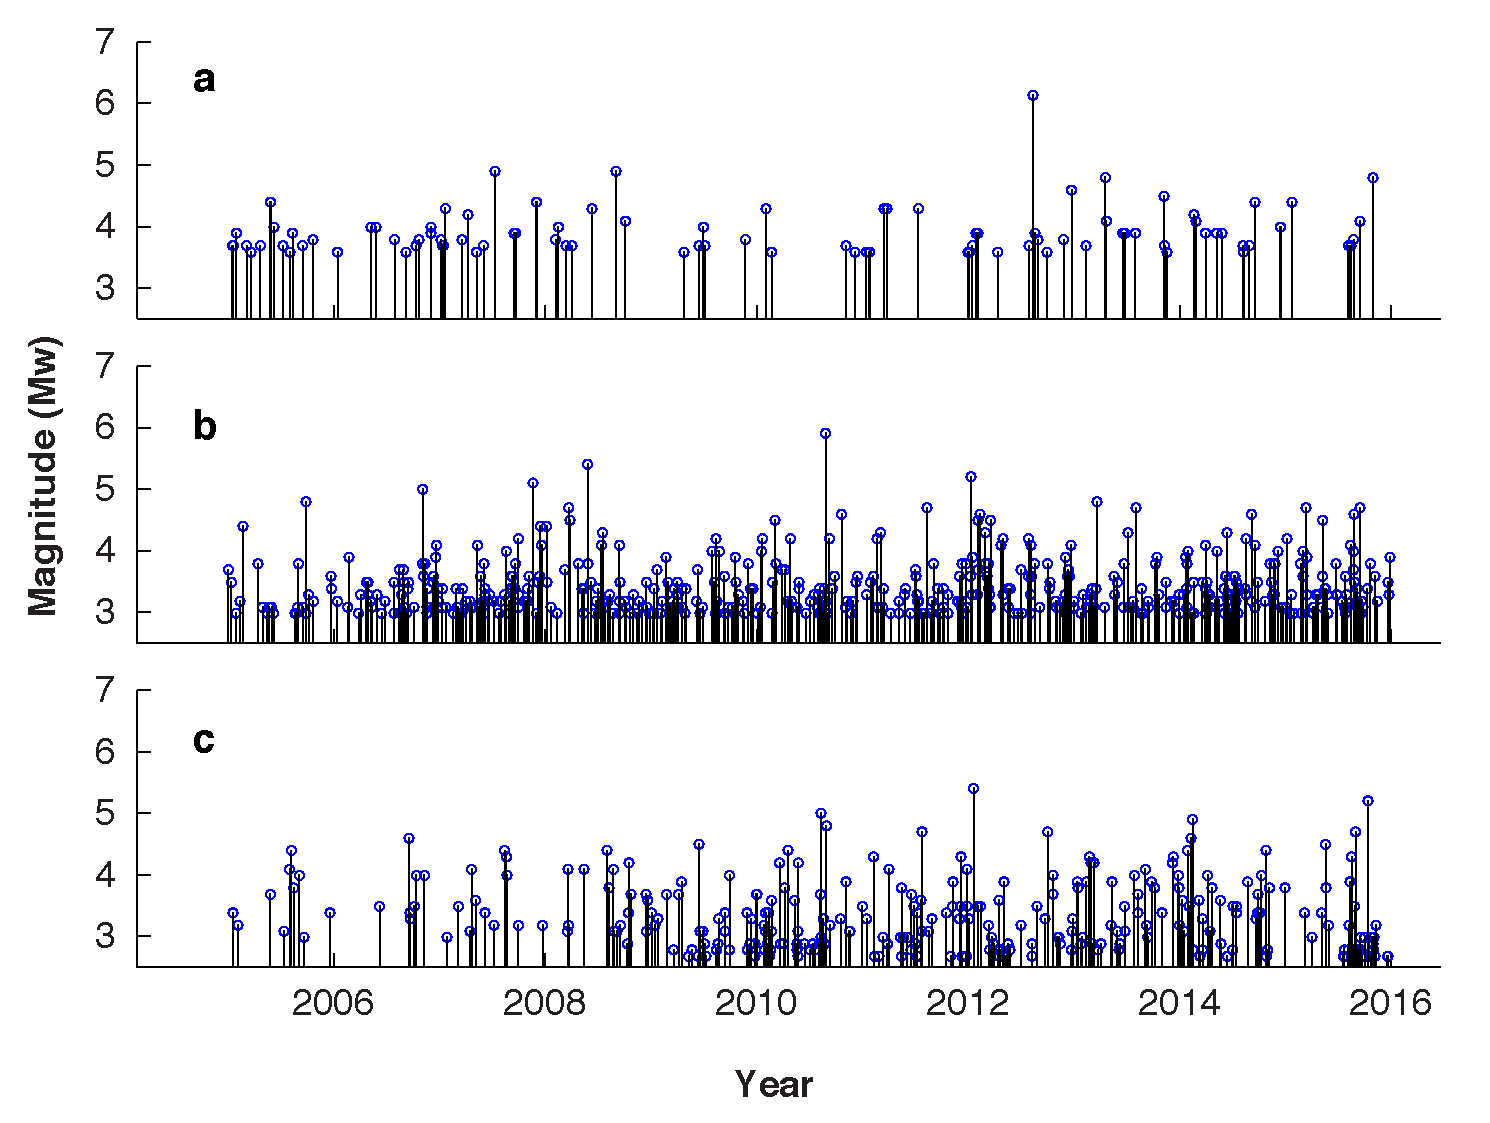
\includegraphics[scale=0.4]{figures/pdf/Figure04.pdf} 
\caption{ Selection of completeness magnitude $M_c$ of the three tectonic seismic regions in northern Iran in 2005-15 period. The symbols indicate the computed GFT values as function of the earthquake magnitude. The horizontal dashed line indicates the desired threshold for the goodness of fit value at 90 percent.}
\label{fig:completeness}
\end{figure} 
\noindent
Based on the results represented in Fig.~\ref{fig:completeness}, we select the minimum magnitudes for complete recording,  $M_c$ , is 3.5, 2.6, and 2.6 for Azerbaijan, Alborz, and Kopeh Dagh, respectively. Fig.~\ref{fig:mag-time}  shows the magnitude time series of the declustered data for the three regions. Earthquakes with magnitude greater than the completeness magnitude are represented. 

\begin{figure} [ht]
\centering
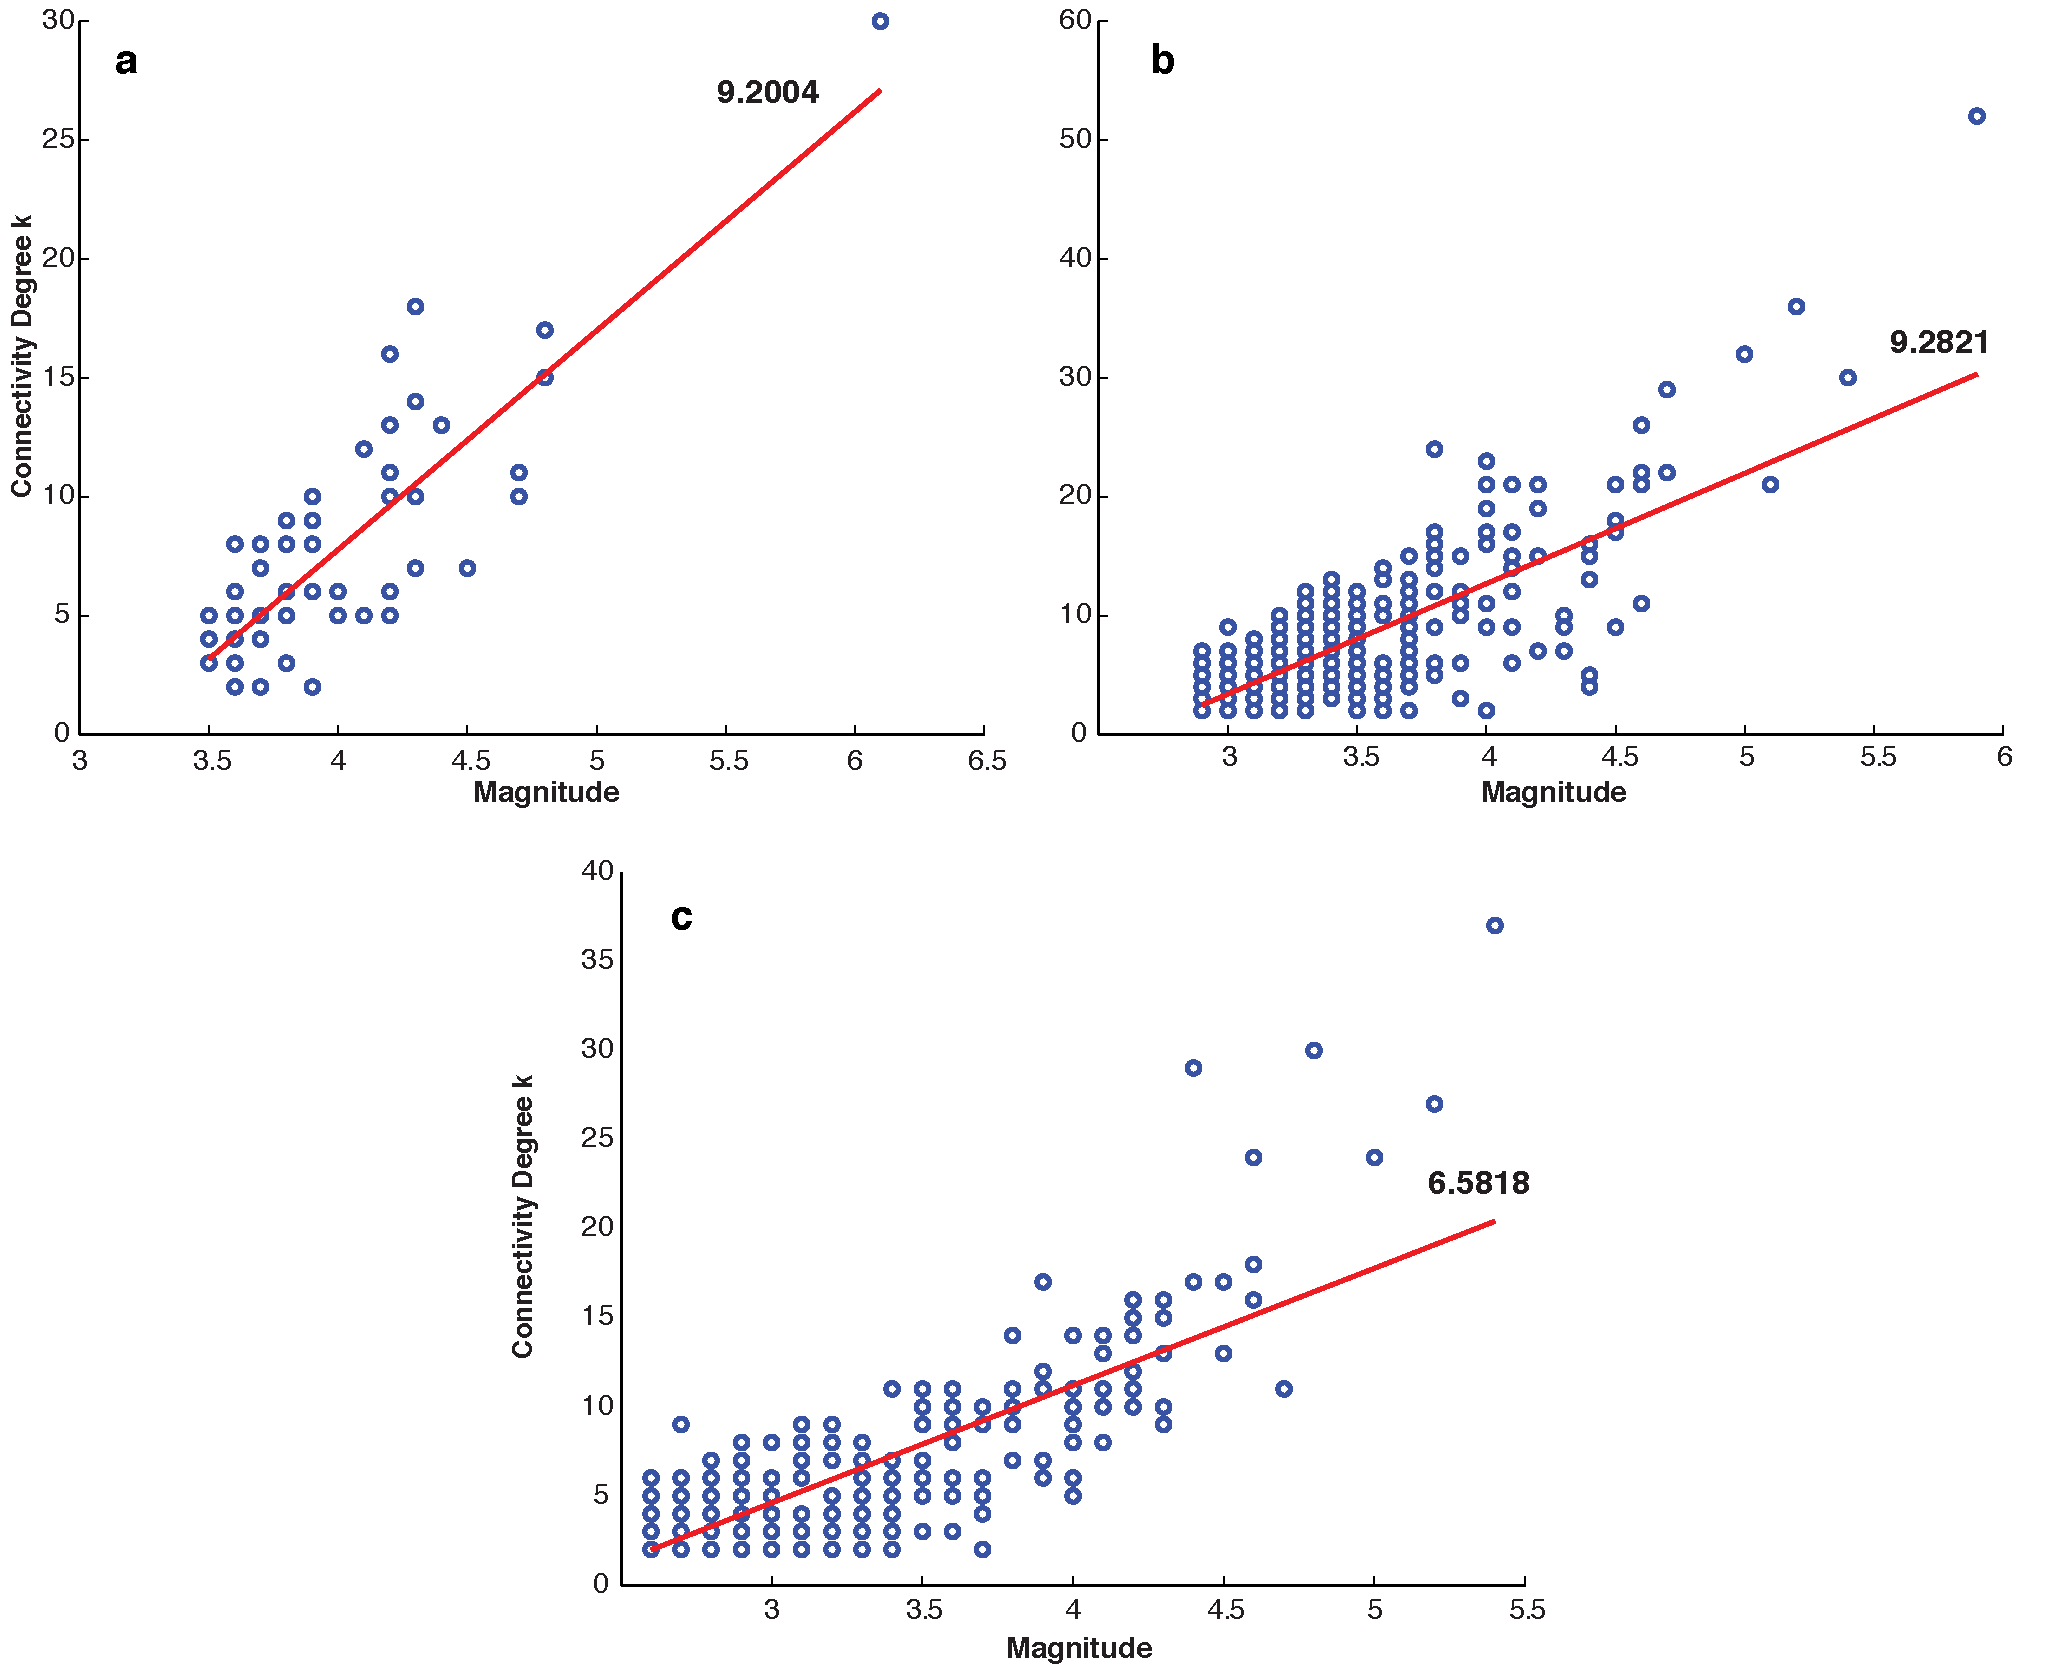
\includegraphics[scale=0.8]{figures/pdf/Figure05.pdf} 
\caption{Variation of moment magnitude ($M_w$) of 2005-2015 earthquake for north Iran as a function of time. The figure only represents the declustered events greater than minimum magnitude. The 2012 $M_w 6.4$ East Azerbaijan, 2010 $M_w 5.8$ Damghan, and 2012 $M_w 5.4$ Neyshabur earthquakes are clearly visible as maximum values in Azerbaijan (Az),  Alborz (Az), and Kopeh Dagh (Ko) magnitude-time series.}
\label{fig:mag-time}
\end{figure} 

 


% Original text
%\section{Tectonic seismic regions and seismicity parameters}
%\noindent
%Iran is situated over Himalayan-Alpide seismic belt, which has frequently experienced strong shaking induced by earthquakes. Based on seismicity parameters, different tectonic seismic devisions have been defined for Iran.  Some studies defined more detailed division \citep{Nowroozi1976, Tavakoli1999}, and some of them defined one simplified province \citep{Stocklin1968, Takin1972, Berberian1976}. \citet{Mirzaei1998} divided Iran into five tectonic regions, including Azerbaijan-Alborz, Kopeh-Dagh, Zagros, Central-East Iran, and Makran. Considering \citet{Mirzaei1998} devision as a reference, \citet{Karimiparidari2013} divided the Azerbaijan-Alborz tectonic seismic region into two regions, which are Azerbaijan and Alborz Mountain Range (hereinafter, Alborz). Azerbaijan, Alborz and Kopeh-Dagh tectonic seismic regions encompass most of the northern Iran.  Fig.~\ref{fig:study_region} shows the study area and tectonic seismic regions. \\
%
%\begin{figure} [ht]
%\centering
%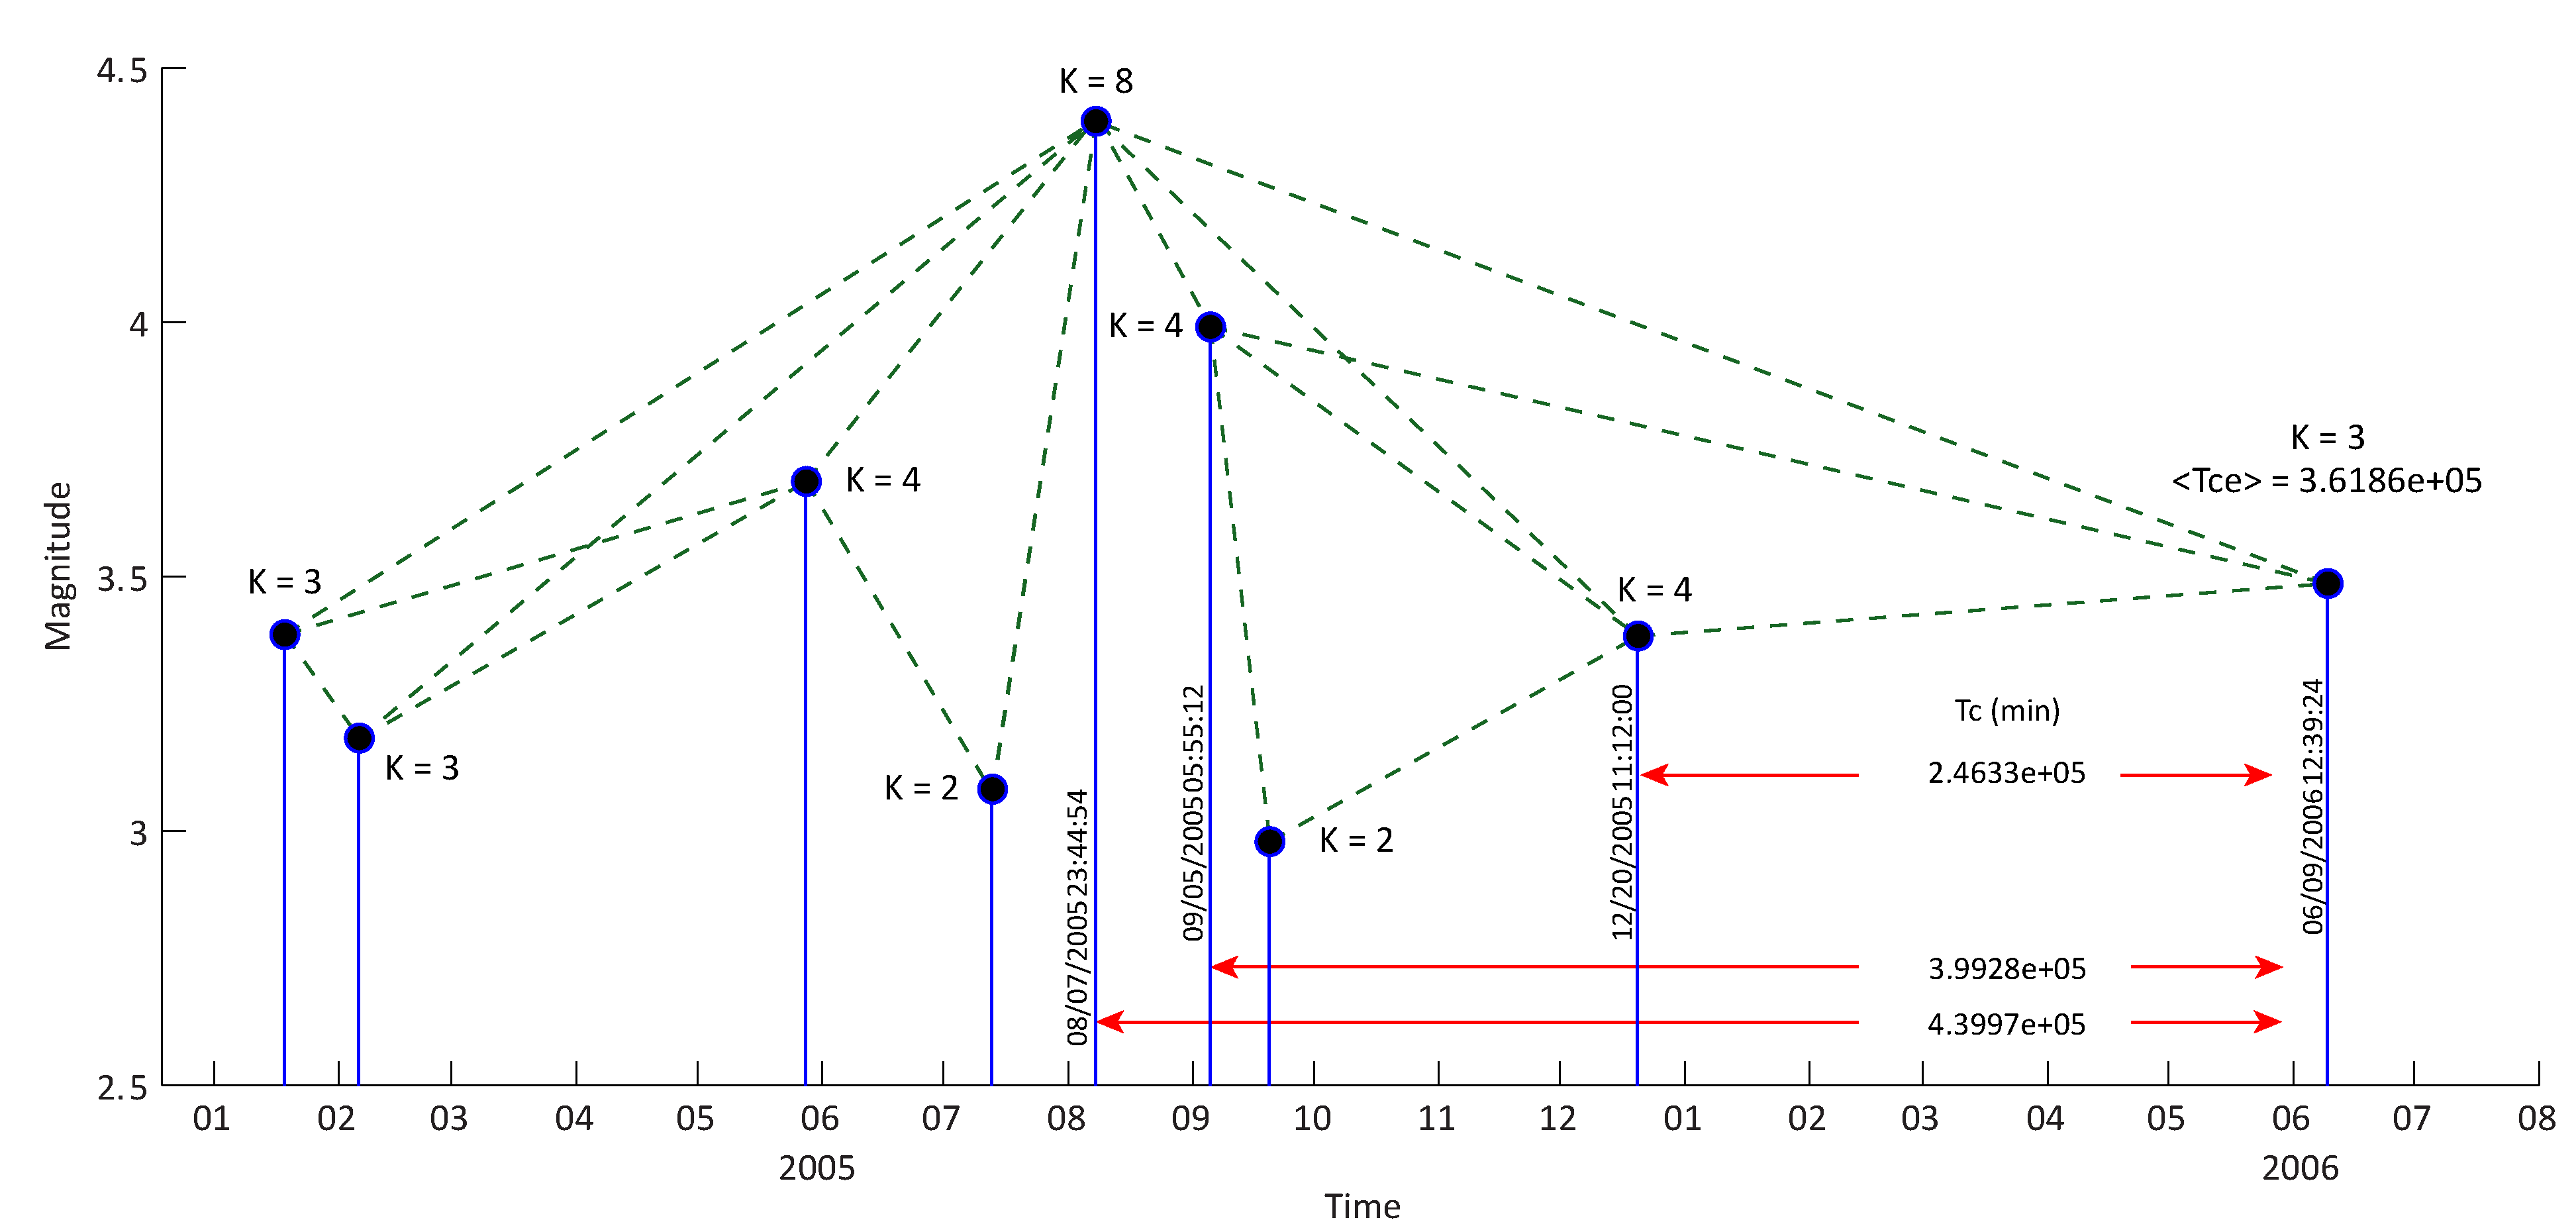
\includegraphics[scale=0.6]{figures/pdf/Figure01.pdf} 
%\caption{a) Map of Iran and surrounding countries. The study area is situated in the gray box. b) The study area containing seismotectonic provinces after \citet{Mirzaei1998} is presented, and location of big cities indicated with circles. Dashed line is the subdivision that is proposed by \citet{Karimiparidari2013}}
%\label{fig:study_region}
%\end{figure}
%
%
%
%
%\noindent
%Alborz tectonic seismic region has active reverse faults, which are parallel to the northwest-trending structural gain of the Alborz Mountains belt. The North Tehran Thrust (NTT) adds more complexity due to the presence of south-dipping reverse faults, which are in part blind, such as the Davudieh, Shian, and Bagh-E Feyz.
%The northwest continuation of the Alborz Mountains, known as the Rocks of the Talesh Mountains, have been thrust northeastward and eastward over rocks of the south Caspian depression \citep{Berberian1999}. 
%
%\noindent
% The Tabriz region (located in Azerbaijan tectonic seismic region) is in the Araxes structural block of northwestern Iran, southwest of the continuation of the western Alborz Mountains towards the Caucasus. The North Tabriz Fault (NTF) is a complex northwest-trending structure, which contains evidence observed on aerial photographs, and vertical displacement with the north side up, of right-lateral strike-slip displacement \citep{Berberian1999}.
%\noindent
%The main Kopeh-Dagh fault consists of several partly overlapping segments parallel to the overall $NW - SE$ structure with step-overs. The regions of overlap are characterized by shorter south-dipping thrust faults striking about E - W \citep{Berberian2001}. \citet{Trifonov1978} reported active displacement along the main Kopeh-Dagh fault for more than 500 km. 
%
%\subsection{Magnitude Conversion}
%\noindent
%The catalog of recorded earthquakes from 2005-2015, which is downloaded from IIEES, reported the earthquakes based on different magnitude scales \citep{IIEES}. We converted the $M_L$, $M_S$, and $mb$ magnitudes through conversion relationships which are defined in \citet{Zare2014}. There are also some of data recorded in $M_D$ (Duration magnitude). These data are reported by International Seismological Centre (ISC).  \citet{Deniz2010} developed a set of empirical equations to convert earthquake magnitudes from $mb$, $M_D$, $M_L$ and $M_S$ scales to $M_W$ scales using orthogonal regression procedure. They used data of earthquake that occurred in Turkey from different data centers including ISC. In this study we use the conversion equation of \citet{Deniz2010} to convert the $M_D$ to $M_W$. 
%
%\subsection{Declustering}
%\noindent
%It is generally assumed that the seismicity of each tectonic seismic source follows a Poissonian occurrence process. Therefore, in order to accomplish this, we declustered the earthquake catalog. In compiling the catalog of events, foreshocks and aftershocks were removed using a declustering methodology \citet{Gardner1974}. Fig.~\ref{fig:seismicity} shows the epicenter of declustered instrumental  earthquakes.
%
%\begin{figure} [ht]
%\centering
%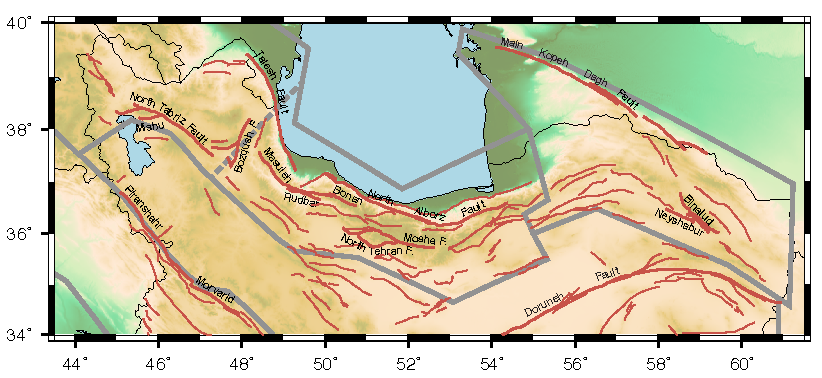
\includegraphics[scale=0.6]{figures/pdf/Figure02.pdf} 
%\caption{Declustered instrumental seismicity map (2005 - 2015) of Northern Iran.}
%\label{fig:seismicity}
%\end{figure}
%
%
%\subsection{Catalog Completeness}
%\noindent
%Completeness of catalog is an important factor in studying the earthquake sequence.  In this study we used the Maximum curvature method (MAXC) \citep{Wiemer2000} to determine the completeness magnitude. According to MAXC method, a complete catalog should follow the Gutenberg-Richter power law distribution of magnitude. The steps for picking the completeness magnitude for each catalog include: 1) Calculating the $a-$ and $b-$ value based on the minimum magnitude, 2) generating  synthetic events based on the achieved value somehow the cumulative number of events obey the power law distribution, and 3) Calculating the goodness of fit for predicted and observed cumulative numbers for each magnitude bin \citep{Wiemer2000}. We increase the minimum magnitude and repeat the process in order to calculate the goodness of fit for each magnitude. \citet{Wiemer2000} assumed the goodness of fit of 90\% as a threshold to select completeness of the catalog. However,  not all frequency-magnitude distributions reach the 90\% mark. Fig.~\ref{fig:completeness} , shows the goodness of fit values for three tectonic seismic regions. For each tectonic seismic region, we pick the magnitude corresponding to the highest goodness of fit or the first magnitude with goodness of fit bigger than 90\%.
%
%\begin{figure} [ht]
%\centering
%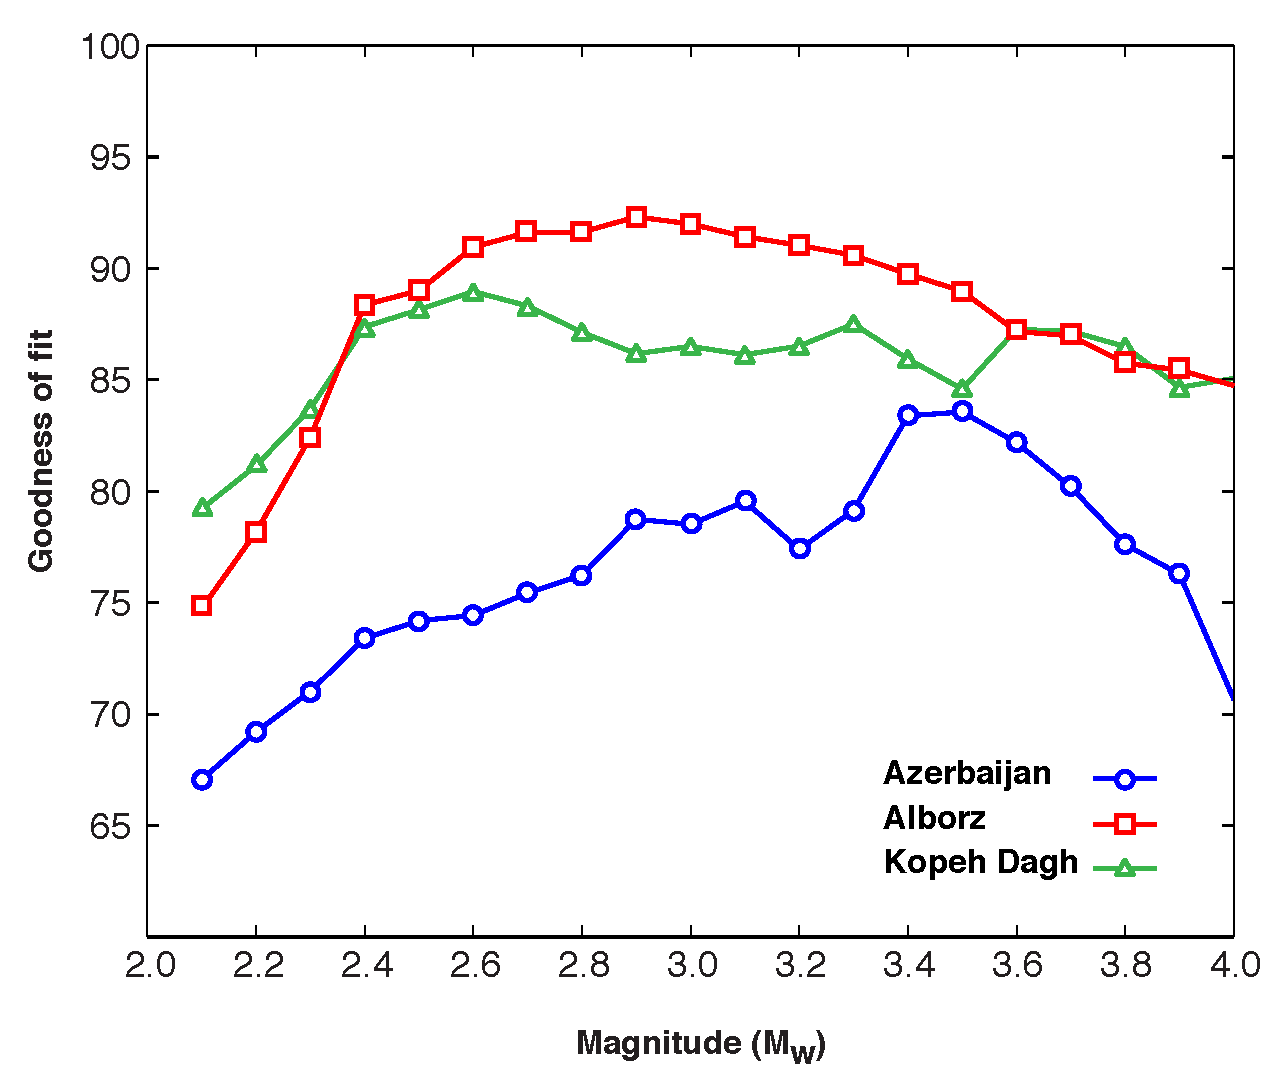
\includegraphics[scale=0.4]{figures/pdf/Figure03.pdf} 
%\caption{Goodness of fit value of MAXC method for three tectonic seismic regions for seismicity of 2005-2015 (a) Azerbaijan b)Alborz c) Kopeh Dagh)}
%\label{fig:completeness}
%\end{figure} 
%
%
%
%
%
%\noindent
%In this study we assume the minimum magnitudes for complete recording, $M_C$, are 3.5, 2.6, and 2.6 for Azerbaijan, Alborz, and Kopeh Dagh, respectively. Fig.~\ref{fig:mag-time} shows the magnitude time series of the declustered data for the three regions. Earthquakes with magnitude bigger than completeness magnitude are represented. 
%
%\begin{figure} [ht]
%\centering
%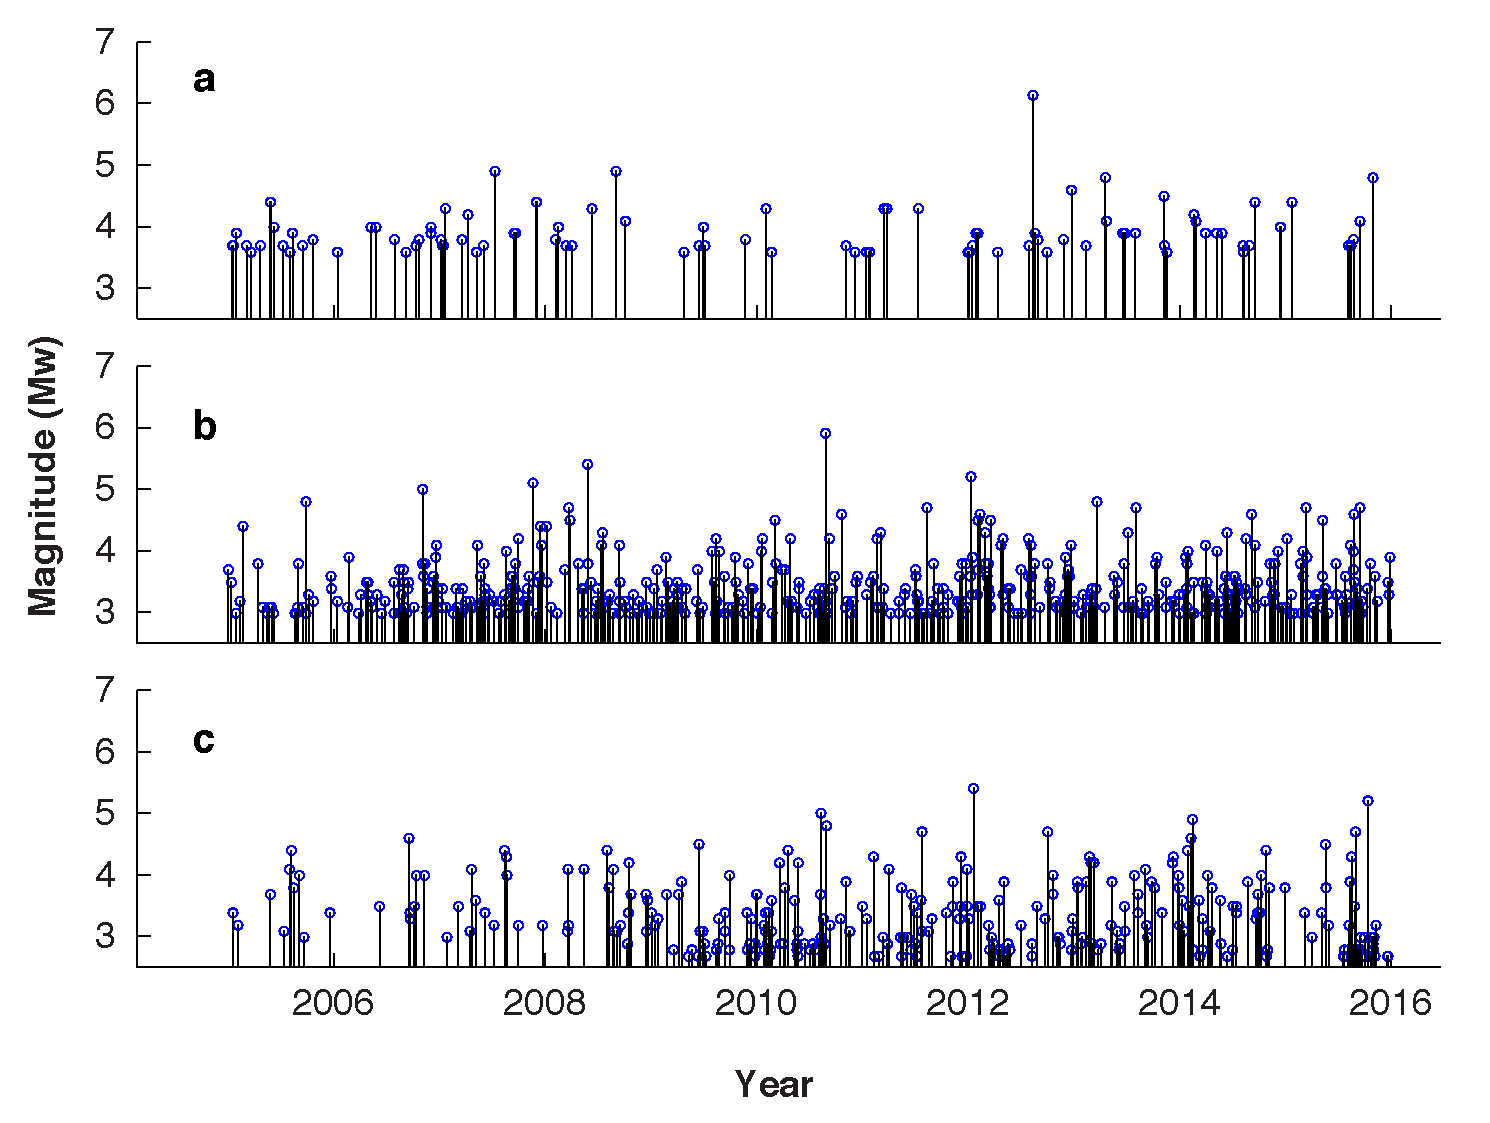
\includegraphics[scale=0.5]{figures/pdf/Figure04.pdf} 
%\caption{Variation of moment magnitude of 2005-2015 earthquake for north Iran. (a) Azerbaijan b)Alborz c) Kopeh Dagh)}
%\label{fig:mag-time}
%\end{figure} 








